\documentclass{standalone}
\usepackage{tikz}
\usetikzlibrary{patterns}
\usetikzlibrary{positioning}
\usetikzlibrary{patterns, positioning}
\usetikzlibrary{shapes.misc}
\usepackage[outline]{contour}
\contourlength{1.5pt} 
\usepackage[sfdefault]{ClearSans}

\begin{document}
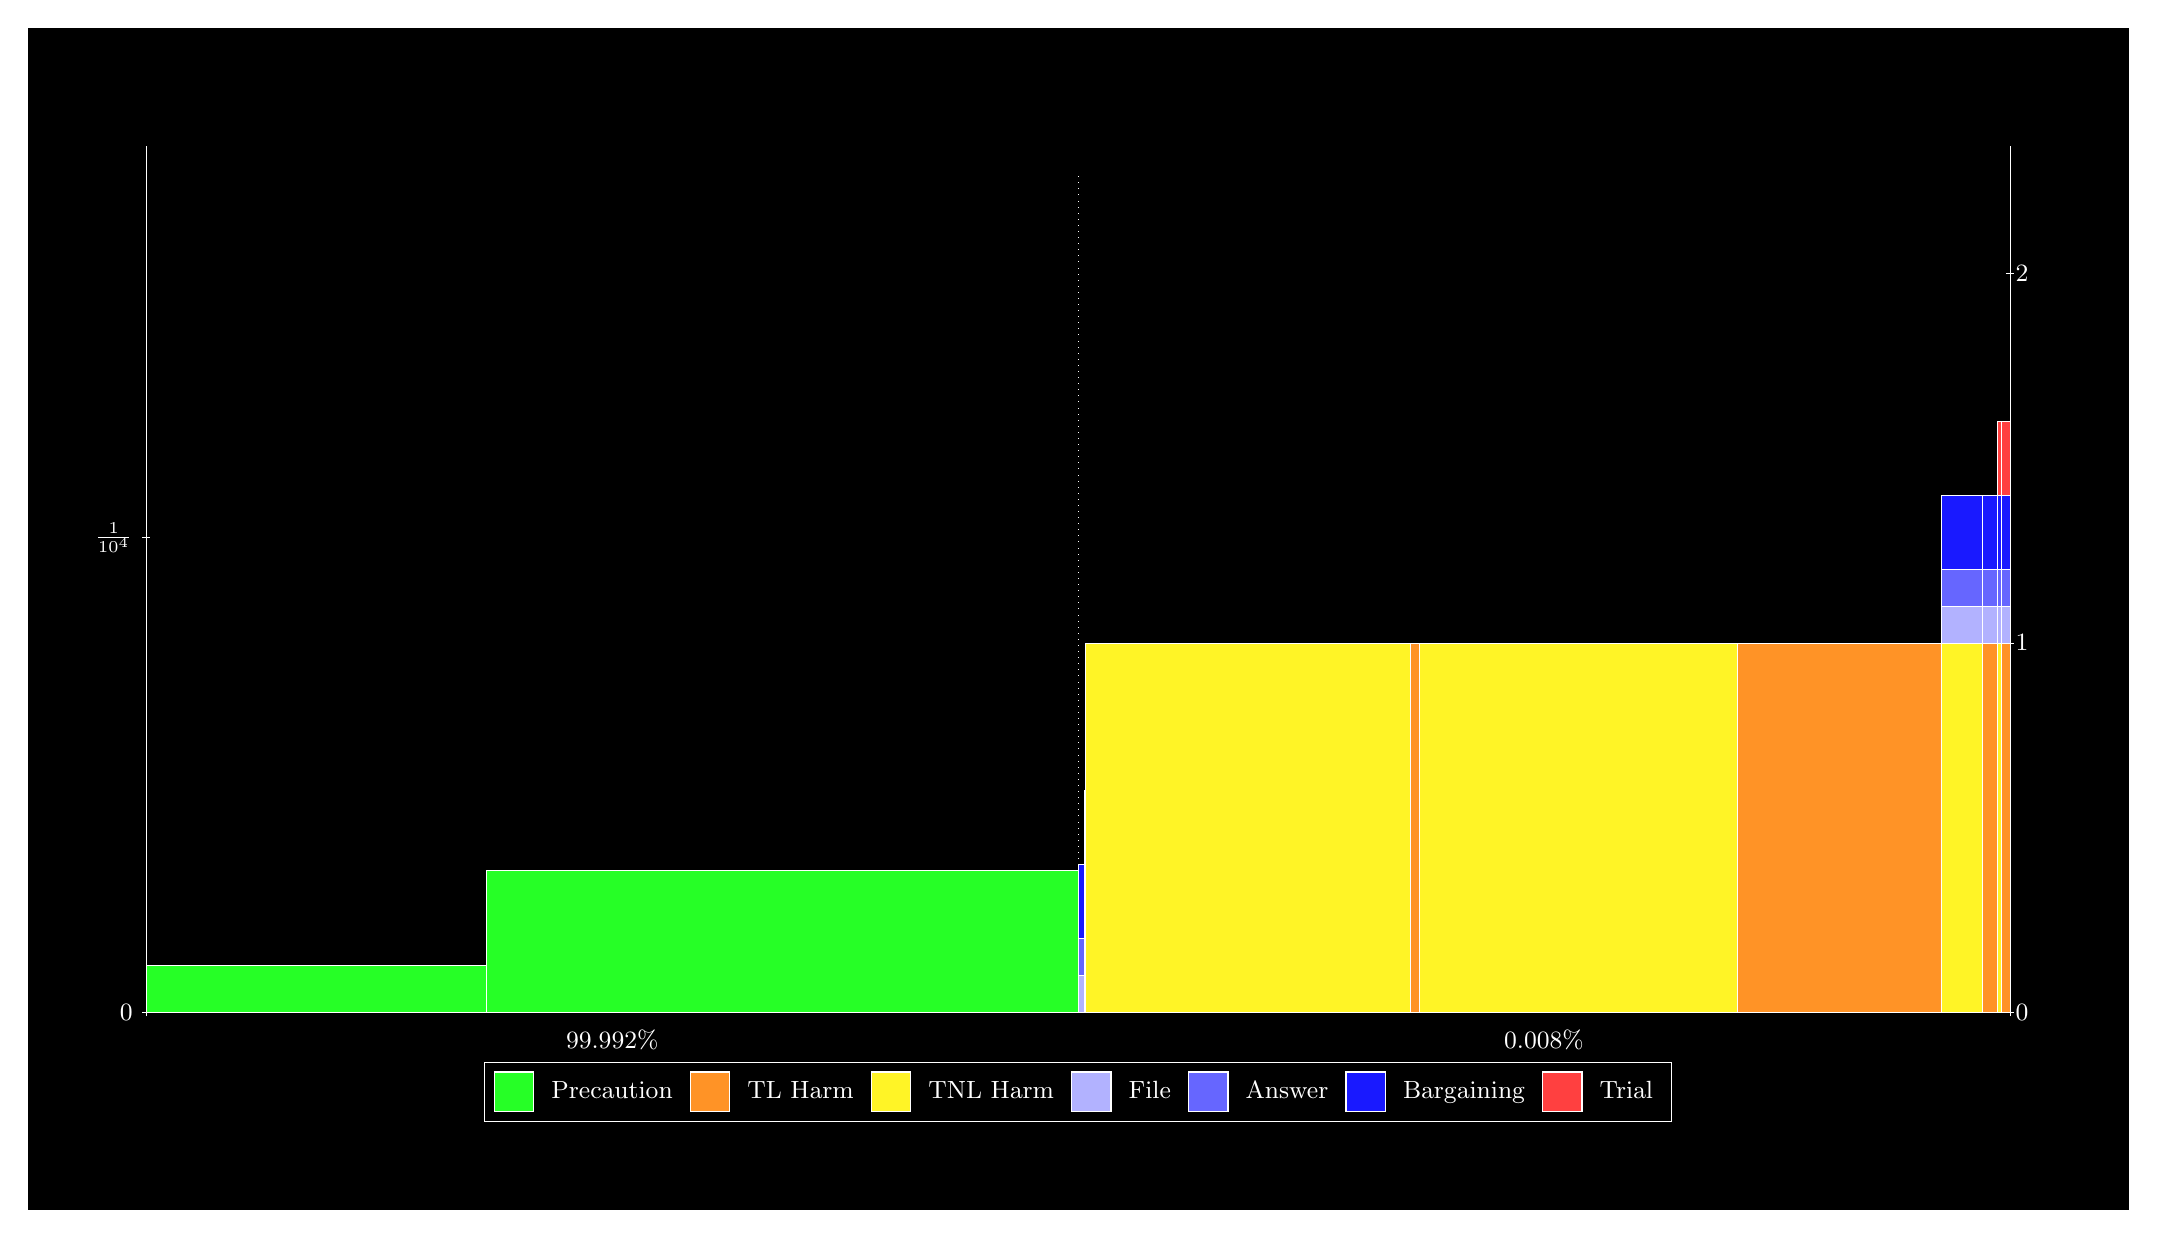
\begin{tikzpicture}
\draw[fill=black] (0,0) rectangle (26.667,15);
\draw[fill=green!85,draw=white,very thin] (1.5,2.5) rectangle (5.8206,3.103);
\draw[fill=green!85,draw=white,very thin] (5.8206,2.5) rectangle (13.333,4.3089);
\draw[fill=green!85,draw=white,very thin] (13.333,2.5) rectangle (13.412,2.5);
\draw[fill=blue!30,draw=white,very thin] (13.333,2.5) rectangle (13.412,2.9694);
\draw[fill=blue!60,draw=white,very thin] (13.333,2.9694) rectangle (13.412,3.4387);
\draw[fill=blue!90,draw=white,very thin] (13.333,3.4387) rectangle (13.412,4.3774);
\draw[fill=green!85,draw=white,very thin] (13.412,2.5) rectangle (13.43,2.5);
\draw[fill=blue!30,draw=white,very thin] (13.412,2.5) rectangle (13.43,2.9694);
\draw[fill=blue!60,draw=white,very thin] (13.412,2.9694) rectangle (13.43,3.4387);
\draw[fill=blue!90,draw=white,very thin] (13.412,3.4387) rectangle (13.43,4.3774);
\draw[fill=red!75,draw=white,very thin] (13.412,4.3774) rectangle (13.43,5.3161);
\draw[fill=green!85,draw=white,very thin] (13.43,2.5) rectangle (17.552,2.5);
\draw[fill=yellow!85,draw=white,very thin] (13.43,2.5) rectangle (17.552,7.1936);
\draw[fill=green!85,draw=white,very thin] (17.552,2.5) rectangle (17.669,2.5);
\draw[fill=orange!85,draw=white,very thin] (17.552,2.5) rectangle (17.669,7.1936);
\draw[fill=green!85,draw=white,very thin] (17.669,2.5) rectangle (21.699,2.5001);
\draw[fill=yellow!85,draw=white,very thin] (17.669,2.5001) rectangle (21.699,7.1936);
\draw[fill=green!85,draw=white,very thin] (21.699,2.5) rectangle (24.295,2.5001);
\draw[fill=orange!85,draw=white,very thin] (21.699,2.5001) rectangle (24.295,7.1936);
\draw[fill=green!85,draw=white,very thin] (24.295,2.5) rectangle (24.81,2.5);
\draw[fill=yellow!85,draw=white,very thin] (24.295,2.5) rectangle (24.81,7.1936);
\draw[fill=blue!30,draw=white,very thin] (24.295,7.1936) rectangle (24.81,7.6629);
\draw[fill=blue!60,draw=white,very thin] (24.295,7.6629) rectangle (24.81,8.1323);
\draw[fill=blue!90,draw=white,very thin] (24.295,8.1323) rectangle (24.81,9.071);
\draw[fill=green!85,draw=white,very thin] (24.81,2.5) rectangle (25.006,2.5);
\draw[fill=orange!85,draw=white,very thin] (24.81,2.5) rectangle (25.006,7.1936);
\draw[fill=blue!30,draw=white,very thin] (24.81,7.1936) rectangle (25.006,7.6629);
\draw[fill=blue!60,draw=white,very thin] (24.81,7.6629) rectangle (25.006,8.1323);
\draw[fill=blue!90,draw=white,very thin] (24.81,8.1323) rectangle (25.006,9.071);
\draw[fill=green!85,draw=white,very thin] (25.006,2.5) rectangle (25.06,2.5);
\draw[fill=yellow!85,draw=white,very thin] (25.006,2.5) rectangle (25.06,7.1936);
\draw[fill=blue!30,draw=white,very thin] (25.006,7.1936) rectangle (25.06,7.6629);
\draw[fill=blue!60,draw=white,very thin] (25.006,7.6629) rectangle (25.06,8.1323);
\draw[fill=blue!90,draw=white,very thin] (25.006,8.1323) rectangle (25.06,9.071);
\draw[fill=red!75,draw=white,very thin] (25.006,9.071) rectangle (25.06,10.01);
\draw[fill=green!85,draw=white,very thin] (25.06,2.5) rectangle (25.167,2.5);
\draw[fill=orange!85,draw=white,very thin] (25.06,2.5) rectangle (25.167,7.1936);
\draw[fill=blue!30,draw=white,very thin] (25.06,7.1936) rectangle (25.167,7.6629);
\draw[fill=blue!60,draw=white,very thin] (25.06,7.6629) rectangle (25.167,8.1323);
\draw[fill=blue!90,draw=white,very thin] (25.06,8.1323) rectangle (25.167,9.071);
\draw[fill=red!75,draw=white,very thin] (25.06,9.071) rectangle (25.167,10.01);
\draw[white,very thin] (1.5,2.5) -- (1.5,13.5);
\draw[white,very thin] (1.45,2.5) -- (1.55,2.5);
\node[font=\small,text=white, anchor=east] at (1.45, 2.5) {0};
\draw[white,very thin] (1.45,8.5296) -- (1.55,8.5296);
\node[font=\small,text=white, anchor=east] at (1.45, 8.5296) {$\frac{1}{10^{4}}$};

\draw[white,dotted,very thin] (13.333,2.83) -- (13.333,13.17);
\draw[white,very thin] (25.167,2.5) -- (25.167,13.5);
\draw[white,very thin] (25.117,2.5) -- (25.217,2.5);
\node[font=\small,text=white, anchor=west] at (25.117, 2.5) {0};
\draw[white,very thin] (25.117,7.1935) -- (25.217,7.1935);
\node[font=\small,text=white, anchor=west] at (25.117, 7.1935) {1};
\draw[white,very thin] (25.117,11.887) -- (25.217,11.887);
\node[font=\small,text=white, anchor=west] at (25.117, 11.887) {2};

\draw[white,very thin] (1.5,2.5) -- (25.167,2.5);
\draw[white,very thin] (1.5,2.45) -- (1.5,2.55);
\node[font=\small,text=white, anchor=north] at (1.5, 2.45) {};
\draw[white,very thin] (25.167,2.45) -- (25.167,2.55);
\node[font=\small,text=white, anchor=north] at (25.167, 2.45) {};

\node[font=\small,text=white,anchor=south] at (7.4167, 1.9) {99.992\%};
\node[font=\small,text=white,anchor=south] at (19.25, 1.9) {0.008\%};
\draw (13.3333,2.5) node (B) {};
\begin{scope}[align=center]
\matrix[scale=0.5,draw=white,below=0.5cm of B,nodes={draw},column sep=0.1cm]{
\node[rectangle,draw,minimum width=0.5cm,minimum height=0.5cm,fill=green!85]{}; & \node[draw=none,font=\small,text=white]{Precaution}; &
\node[rectangle,draw,minimum width=0.5cm,minimum height=0.5cm,fill=orange!85]{}; & \node[draw=none,font=\small,text=white]{TL Harm}; &
\node[rectangle,draw,minimum width=0.5cm,minimum height=0.5cm,fill=yellow!85]{}; & \node[draw=none,font=\small,text=white]{TNL Harm}; &
\node[rectangle,draw,minimum width=0.5cm,minimum height=0.5cm,fill=blue!30]{}; & \node[draw=none,font=\small,text=white]{File}; &
\node[rectangle,draw,minimum width=0.5cm,minimum height=0.5cm,fill=blue!60]{}; & \node[draw=none,font=\small,text=white]{Answer}; &
\node[rectangle,draw,minimum width=0.5cm,minimum height=0.5cm,fill=blue!90]{}; & \node[draw=none,font=\small,text=white]{Bargaining}; &
\node[rectangle,draw,minimum width=0.5cm,minimum height=0.5cm,fill=red!75]{}; & \node[draw=none,font=\small,text=white]{Trial}; \\\\
};\end{scope}

\end{tikzpicture}
\end{document}